\ifsolo
~

\vspace{1cm}

\begin{center}
\textbf{\LARGE Compléments sur les polynômes} \\[1em]
\end{center}
\fi


\ifsolo
\tableofcontents
\else
\chapter{Compléments sur les polynômes}
\fi

Tous les théorèmes ou propositions présents dans ce chapitre sont soit déjà connus (donc au programme) soit nouveaux et sont alors des compléments de cours (hors programme). Le chapitre dans sa totalité n'est pas au programme, seuls quelques rappels du programme y sont présents car pertinents et/ou utiles au développement d'autres compléments.
\ifsolo
\else
\minitoc
\fi
\thispagestyle{empty}

\ifsolo \newpage \setcounter{page}{1} \fi
\section{Rappels}

$\K$ désigne un corps (donc commutatif). Un polynôme de $\K[X]$ s'écrit $P$ ou $P(X)$, l'évaluation en $a\in\K$ de $P$ se note $P(a)$. L'application \[
    P\in\K[X] \longmapsto (a\longmapsto P(a)\in\K)
\]
est un morphisme d'algèbres qui est injectif si $\K$ est infini. Pour $P\in\K[X]\setminus \{0\}$, $a\in\K$ est une racine de $P$ ssi \[
    P(a)=0\iff (X-a)\;|\;P
\]
et $a$ est racine de multiplicité $\alpha \geq 1$ ssi \[
    \begin{cases}
        P(a)=P'(a)=\cdots=P^{(\alpha - 1)}(a)=0 \\
        P^{(\alpha)}(a)\neq 0
    \end{cases}
    \iff \begin{cases}
        (X-a)^\alpha \; |\; P\\
        (X-a)^{\alpha+1}\;\not|\;P
    \end{cases}
\]
Si $a$ n'est pas racine de $P$, on convient que $a$ est racine de multiplicité $0$.

\begin{notation} ~
    \begin{itemize}
        \item
            On note $Z_\K(P)$ l'ensemble des racines de $P$ dans $\K$
        \item On note $\mathrm{mult}(P, a)$ la multiplicité de la racine $a$ dans $P$
    \end{itemize}
\end{notation}

\begin{thm}
    Soit $P\in \K[X]\setminus \{0\}$. Le polynôme $P$ a au plus $\deg P$ racines dans $\K$.
    En particulier, le polynôme nul est le seul polynôme qui a une infinité de racines.
\end{thm}

\begin{thm}
    Soit $P\in\K[X]$.
    \begin{enumerate}
        \item \[
                P(X)=\sum_{k=0}^{+\infty} \frac{P^{(k)}(0)}{k!}X^k
            \]
        \item \[
                \forall a\in\K, \quad P(X)=\sum_{k=0}^{+\infty}\frac{P^{(k)}(a)}{k!}(X-a)^k
            \]
    \end{enumerate}
\end{thm}
\begin{proof} ~
    \begin{enumerate}
        \item L'application \[
                \psi: P\longmapsto P(X)-\sum_{k=0}^{+\infty}\frac{P^{(k)}(a)}{k!}(X-a)^k
            \]
            est linéaire nulle sur les vecteurs de la base canonique.
    \end{enumerate}
\end{proof}

\begin{rem}
    On montre de même que \[
        P(a)=\sum_{k=0}^{+\infty}\frac{P^{(k)}(X)}{k!}(a-X)^k
    \]
\end{rem}

\section{Factorisation des polynômes}

\subsection{Rappels}

\begin{thm}
    Soit $P\in\K[X]$, $a_1, \cdots, a_p$ deux à deux distincts et $n_1, \cdots, n_p\in\N^\star$. Si $a_1, \cdots, a_p$ sont des racines de multiplicités $n_1, \cdots, n_p$ de $P$, alors \[
        (X-a)^{n_1}\cdots (X-a_p)^{n_p}\;|\;P
    \]
    En particulier, si $\deg P=\sum_i n_i$ alors il existe $\lambda\in\K^\star$ tel que \[
        P(X)=\lambda(X-a_1)^{n_1}\cdots (X-a_p)^{n_p}
    \]
\end{thm}

\subsection{Théorème de d'Alembert-Gauss}

\begin{thm}[D'Alembert-Gauss] \index{D'Alembert-Gauss (théorème de -- )}
    Tout polynôme non constant de $\C[X]$ admet au moins une racine
\end{thm}

\begin{proof}[Preuve de Gauss]
    \begin{itemize}
        \item $P\in \C[X]$ non constant a même racine que $\frac1{\deg P}P$ donc on suppose $P$ unitaire.
        \item Si $P(X)=a_0+\cdots+ a_{n-1}X^{n-1}+X^n$, et $M=\max |a_i|$, alors pour $|z|\geq M+2$, \begin{align*}
                |P(z)|&\geq |z|^n-M\frac{|z|^n-1}{|z|-1}=\frac{|z|^{n+1}-|z|^n-M|z|^n+M}{|z|-1}\\
                      &\geq \frac{|z|^n}{|z|-1} \left( |z|-1-M \right)\geq |z|^n\left(1-\frac M{M+1}\right)\geq \frac{(M+2)^n}{M+1}>M
            \end{align*}
        \item \begin{align*}
                \inf_{\C}|P|&=\min\left(\underbrace{\inf_{|z|>M+2}|P(z)|}_{>M}, \underbrace{\inf_{|z|\leq M+2}|P(z)|}_{\leq |P(0)|\leq M}\right) \\&=\inf _{|z|\leq M+2}|P(z)|
            \end{align*}
            Par compacité il existe $z_0\in\mathcal B_f(0, M+2)$ tel que $\inf_{\C}|P|=|P(z_0)|$.
        \item Si $P(z_0)\neq 0$ alors il existe $k\geq 1$ tel que \begin{align*}
                P(z_0+h)&=P(z_0)+\frac{P^{(k)}(z_0)}{k!}h^k+o(h^k), \quad P(z_0)\neq 0 \\
                        &=P(z_0)\left(1+h^k\frac{P^{(k)}(z_0)}{P(z_0)k!}+o(h^k) \right)
            \end{align*}
        \item En écrivant \[
                \frac{P^{(k)}(z_0)}{P(z_0)k!}=\rho e^{i\theta}, \quad h=\epsilon e^{-i\frac{\theta+\pi}k}
            \]
            on obtient \[
                P(z_0+\epsilon e^{-i\frac\theta k})=\underbrace{P(z_0)\underbrace{\left(1 - \epsilon^k \rho + o(\epsilon^k)\right)}_{|\;\;|<1}}_{|\;\;|<|P(z_0)|}
            \]
            absurde.
    \end{itemize}
\end{proof}

\section{Polynômes sous contraintes}

\subsection{Contraintes sur les zéros}

\begin{exo}
    Si $Z_{\C}(P)=Z_{\C}(Q)$ et $Z_{\C}(P+1)=Z_{\C}(Q+1)$ pour $P,Q$ non constants de $\C[X]$, alors $P=Q$
\end{exo}

On suppose par l'absurde que $P\neq Q$ et par exemple $n=\deg P\geq \deg Q=m$. On note $u_1, \cdots, u_r$ les racines de $P$ (et donc de $Q$), $v_1, \cdots, v_s$ les racines de $P+1$ (donc de $Q+1$). Les $u_i$ et les $v_j$ sont tous distincts, donc \[
    \deg P=n\geq \deg(P-Q)\geq r+s \quad\text{car }P-Q\text{ s'annule en $u_i$ et $v_j$ et }P-Q\neq 0
\]
On a $P'=(P+1)'$ donc $P'$ a $n-r$ racines dans les $u_i$ avec multiplicité, et $n-s$ dans les $n_j$ donc \[
    n-r+n-s\leq \deg P'=n-1\iff n+1\leq r + s
\]
Or $r+s\leq n$ absurde et donc $P = Q$

\subsection{Coefficients unitaires}

\begin{exo}
    Déterminer les $P\in\R[X]$ non constants avec les coefficients $\pm1$ et dont toutes les racines sont réelles.
\end{exo}

\begin{proof}[Résolution]
    On note $P$ un polynôme de degré $n\geq 2$ qui convient et quitte à changer $P$ en $-P$, $P$ est unitaire.
    \begin{itemize}
        \item $P(X)=X^n+p_{n-1}X^{n-1}+\cdots +p_0$
        \item $r_1, \cdots, r_n$ les racines (non nulles car $p_0\neq 0$) donne \[
                r_1^2+\cdots +r_n^2=p_{n-1}^2-2p_{n-2}>0 \implies p_{n-2}=-1 \text{ et }r_1^2+\cdots+r_n^2=3
            \]
        \item \[
                p_0 X^n P \left( \frac1X \right)=X^n+p_0p_1X^{n-1}+p_0p_2X^{n-2}+\cdots
            \]
            vérifie les mêmes propriétés donc \[
                \frac 1{r_1^2} +\cdots +\frac1{r_n^2}=3
            \]

        \item \[
                \sum_{i=1}^n\underbrace{\left(r_i^2+\frac1{r_i^2}\right)}_{\geq 2}=6 \implies n\leq 3
            \]
    \end{itemize}
    On doit étudier $12$ polynômes
    \begin{center}
        \begin{tabular}{lll}
            \sout{$X^2+X+1$} & \sout{$X^3+X^2+X+1$} & \sout{$X^3-X^2+X+1$} \\
            $X^2+X-1$ & \sout{$X^3+X^2+X-1$} & \sout{$X^3-X^2+X-1$} \\
            \sout{$X^2-X+1$} & \sout{$X^3+X^2-X+1$} & $X^3-X^2-X+1$ \\
            $X^2-X-1$ & $X^3+X^2-X-1$ & \sout{$X^3-X^2-X-1$}
        \end{tabular}
    \end{center}
\end{proof}

\subsection{Équation fonctionnelle}

\begin{exo}
    Déterminer les polynômes $P\in\C[X]$ tels que $P(X)P(X+2)+P(X^2)=0$
\end{exo}

\begin{proof}[Résolution] $-1$ et $0$ sont les deux polynômes constants solutions.

    Soit $P$ non constant solution et $a$ une racine. $P(a)=0\implies P(a^2)=0$ donc $P$ admet une infinité de racines sauf si $|a|=1$ ou $a=0$.

    Si $a=0$ est racine alors $P(-2)P(0)+P(4)=0$ donc $4$ est racine ce qui est absurde. Donc $|a|=1$.

    Si $a$ est racine alors $(a-2)^2$ racine donc $|a-2|=1=|a|$ donc $a=1$ (intersection de deux cercles), donc $1$ seule racine de $P$ et donc pour un $k\geq 1$, \[
        P=\lambda(X-1)^k
    \]
    En calculant, on trouve $\lambda^2+\lambda=0$ et $\lambda \neq 0$ donc $\lambda = -1$
\end{proof}

\begin{exo}
    Trouver les polynômes $P\in\R[X]$ tels que \[
        (X+1)P(X-1)-(X-1)P(X)
    \]
    est un polynôme constant
\end{exo}

\begin{proof}[Résolution]
    On suppose que $P$ convient et $(X+1)P(X-1)-(X-1)P(X)=\lambda$. \begin{itemize}
        \item $2P(-1)=\lambda$ et $2P(0)=\lambda$ donc $P(0)=P(-1)$
        \item $Q(X)=P(X)-\frac\lambda 2$ s'annule en $-1$ et $0$ donc $Q(X)=X(X+1)A(X)$ i.e.  $P(X)=X(X+1)A(X)+\frac\lambda 2$.
        \item \[
                (X+1)((X-1)X A(X-1)+\frac\lambda2)-(X-1)X(X+1)A(X)-(X-1)\frac\lambda2=\lambda
            \]
            donc \[
                X(X-1)(X+1)(A(X-1)-A(X))=0 \implies A(X)=A(X-1)
            \]
            et donc $A$ est un polynôme constant. Donc $P$ est de la forme $P(X)=aX(X+1)+\mu, \quad a, \mu\in\R$
    \end{itemize}
\end{proof}

\section{Liens coefficients et racines}

\subsection{Relations de Viète}

\index{Viète!relations}

Pour $x_1, \cdots, x_n\in\C$ on note: \[
    \sigma_i(x_1, \cdots, x_n)=\sum_{\substack{I\subset \llbracket 1, n\rrbracket\\|I|=i}}\prod_{l\in I}x_l
\]
Soit $P(X)=a_nX^n+\cdots+a_0$ un polynôme de degré $n$ et $x_1, \cdots, x_n$ ses racines dans $\C$. \begin{itemize}
    \item \begin{align*}
            P(X)=a_n(X-x_1)\cdots (X-x_n)=a_n(X^n-\sigma_1 X^{n-1}+ \sigma_2 X^{n-2}+\cdots (-1)^n\sigma_nX^{n-n})
        \end{align*}
    \item Ainsi, \[
            \forall i\in\llbracket 1, n\rrbracket, \quad (-1)^i\sigma_i=\frac{a_{n-i}}{a_n}
        \]
\end{itemize}
En particulier, on en déduit \[
    x_1+\cdots+x_n = -\frac{a_{n-1}}{a_n}
\]
et \[
    x_1\times \cdots\times x_n=(-1)^n\frac{a_0}{a_n}
\]

\subsection{Somme de Newton}

On note $P(X)=a_nX^n+\cdots+a_0$ un polynôme de $\C[X]$, $x_1, \cdots, x_n$ ses racines. On note $S_k=x_1^k+\cdots + x_n^k$ appelée $k-$ième somme de Newton \index{Newton!sommes}.

Pour $k\geq n$, \begin{align*}
    a_nS_k+a_{n-1}S_{k-1}+\cdots + a_0S_{k-n}&=a_nx_1^k+\cdots +a_0x_1^{k-n}+\cdots +a_nx_n^k+\cdots +a_0x_n^{k-n} \\ &=x_1^{k-n}P(x_1)+\cdots + x_n^{k-n}P(x_n)=0
\end{align*}

Avec les relations de Viète, pour $k\geq n$, \[
    \underbrace{\sigma_0}_{=\; 0 \text{ convention}} S_k-\sigma_1S_{k-1}+\cdots + (-1)^nS_{k-n}=0
\]

Il est possible de calculer $S_1, \cdots, S_{n-1}$ par des formules de récurrence. \begin{itemize}
    \item $S_0=n$ clair. On va montrer que \[
            k\sigma_k=\sum_{i=1}^k(-1)^{i-1}\sigma_{k-i}S_i
        \]
    \item On note $P$ le polynôme $P/\dom P$\[
            P(x)=\prod_{i=1}^n(x-x_i)=\frac1{a_n}\sum_{k=0}^na_kx^k=\sum_{k=0}^n\sigma_{n-k}(-1)^{n-k}x^k
        \]
        d'où \[
            x^nP\left(\frac1x\right)=\underbrace{\prod_{k=1}^n(1-xx_k)}_{Q(x)}=\sum_{k=0}^n\sigma_{n-k}(-1)^{n-k}x^{n-k}=\sum_{k=0}^n\sigma_k(-1)^kx^k
        \]
    \item \begin{align*}
            \sum_{k=0}^n k\sigma_k(-1)^kx^k&= x\sum_{k=1}^n \frac{Q(x)}{1-xxk}(-x_k) \\
                                           &=-\sum_{k=1}^n\frac{xx_k}{1-xx_k}Q(x) \\
                                           &=-\left(\sum_{k=1}^n\sum_{i\geq 0}(xx_k)^{i+1}\right)Q(x) \\
                                           &=-\sum_{i\geq 0}x^{i+1}S_{i+1}\sum_{l=0}^n(-1)^k\sigma_kx^k
        \end{align*}

        En identifiant le coefficient de $x^k$, \begin{align*}
            (-1)^kk\sigma_k=-\sum_{l=0}^{k-1}(-1)^l\sigma_lS_{k-l} \iff k\sigma_k &=-\sum_{l=0}^{k-1}(-1)^{k-l}\sigma_lS_{k-l} \\
                                                                                  & =\sum_{l=1}^k(-1)^{l-1}\sigma_{k-l}S_l
        \end{align*}
\end{itemize}

\section{Polynômes scindés sur $\R$}

\subsection{Une CNS}

\begin{exo}
    Montrer que $P\in\R[X]$ de degré $n$ est scindé sur $\R$ ssi \[
        \forall z\in\C, \quad |P(z)|\geq |\dom(P)|\times |\Im(z)|^n
    \]
\end{exo}

\begin{proof}[Résolution]
    \emph{($\Longrightarrow$)} clair, les racines complexes de $P$ ont une partie imaginaire nulle.

     \emph{($\implies$)} On écrit $P(X)=\dom(P)(X-a_1)\cdots (X-a_n), \quad a_i\in\R$. En injectant $z=a+ib$, \[
        |P(z)|=|\dom P|\times |a-a_1+ib| \cdots |a-a_n+ib|\geq |\dom P| |b|^n
    \]
\end{proof}

\subsection{Opérations stabilisant $\mathcal S$}

On note $\mathcal S$ l'ensemble des polynômes scindés de $\R[X]$. On note \[
    P(X)=\lambda (X-a_i)^{\alpha_1}\cdots (X-a_p)^{\alpha_p}, \quad a_1<\cdots <a_p
\]
et on a les propriétés de stabilité suivantes.

\vspace{.2cm}

 Rolle donne que $P'$ s'annule au moins une fois sur $]a_i, a_{i+1}[$ pour $1\geq i < p$. Il y a alors au total $(\alpha_1-1)+\cdots+(\alpha_p-1)+p-1=n-1$ racines réelles (avec multiplicité) et $\deg P'=n-1$ donc $P'$ est scindé et $\mathcal S$ est stable par dérivation.

\vspace{.2cm}

 Pour $a\in\R$ fixé, on note $g(x)=e^{ax}P(x)$, $g'(x)=(P'(x)+aP(x))e^{ax}$. $P'+aP$ s'annule en $a_i$ avec multiplicité $\geq \alpha_i-1$. Rolle donne que $g'$ s'annule au moins une fois sur $]a_i, a_{i+1}[$ donc $P'+aP$ aussi. Ce polynôme a $n-1$ racines réelles et est de degré $n$, donc par division la dernière racine est réelle. Donc $P'+aP\in\mathcal S$

\vspace{.2cm}

 Plus généralement, si $D$ est l'opérateur de dérivation polynomiale, pour $Q\in\mathcal S$ alors
\begin{itemize}
    \item
\[
    Q(X)=\lambda (X-b_1)\cdots (X-b_p)
\]
\item \[
        Q(D)=\lambda(D-b_1\mathrm{id})\circ \cdots \circ (D-b_p \mathrm{id})
    \]
\end{itemize}
et pour $P\in\mathcal S$, $Q(D)(P)\in\mathcal S$.

\subsection{Faisceau de polynômes à racines entrelacées (ENS)}

\begin{exo}
    On note $P, Q\in\R[X]$ deux polynômes scindés à racines simples distinctes tels qu'entre deux racines de l'un, il y en aie au moins une de l'autre. Montrer que $\lambda P+\mu Q$ est scindé sur $\R$
\end{exo}

\begin{proof}[Résolution]
    On suppose que $P$ a la plus petite racine, on note $x_1 <\cdots<x_n$ les racines de $P$. Sur $]x_1, x_2[$, il y a au moins une racine de $Q$ et au plus une (sinon $x_1$ et $x_2$ ne sont pas consécutives) donc les $n-1$ premières racines de $Q$ satisfont \[
        x_1<y_1<\cdots <x_{n-1}<y_{n-1}<x_n
    \]
    Il y a lors deux cas: $Q$ possède une racine $y_n>x_n$, ou $Q$ a $n-1$ racines réelles. On se place dans le premier cas (l'autre se traite similairement).

    Comme $\lambda, \mu\in\R$ sont quelconques, on peut supposer $P$ et $Q$ unitaires donc \[
        P(X)=(X-x_1)\cdots (X-x_n) \qquad Q(X)=(X-y_1)\cdots (X-y_n)
    \]
    Pour $\lambda, \mu\neq 0$, les racines réelles de $\lambda P+\mu Q$ sont différentes des $x_i, y_i$, donc sont les mêmes que celles de $\frac{\lambda P+\mu Q}{PQ}$ sur $\R\setminus \{x_i, y_i\}$. \[
        \varphi(x)=\frac{\lambda P(x)+\mu Q(x)}{P(x)Q(x)}=\frac\lambda{Q(x)}+\frac\mu{P(x)}
    \]
    Si $\lambda, \mu>0$, alors $\varphi$ s'annule $n$ fois car il y a changement de signe entre $]x_i, y_i[$ (les polynômes sont unitaires donc on connaît exactement les signes de $P$ et $Q$). Si $\lambda>0>\mu$, on trouve $n-1$ racines réelles de la même manière, et par division la dernière est aussi réelle. Les autres cas se traitent de la même manière.
\end{proof}

\section{Valeurs des polynômes}

\subsection{Polynôme à valeurs entières}

On va caractériser les polynômes de $\C[X]$ tels que $P(\Z)\subset \Z$

On définit \[
    \binom X0=1\qquad \text{ et }\qquad \forall n\geq 1,\quad \binom Xn=\frac1{n!}X(X-1)\cdots(X-n+1)
\]

\begin{lmm}
    Pour tout $n\in\N$ et pour tout $x\in\Z$, \[
        \binom xn\in\Z
    \]
\end{lmm}

\begin{proof}
    Pour $0\leq x\leq n-1$, $\binom xn=0$. Pour $x\geq n$, $\binom xn$ est un coef du binôme. Pour $x<0$, $(-1)^n\binom xn$ est un coef du binôme.
\end{proof}

 On introduit \[
    \Delta : P\in\K[X]\longmapsto P(X+1)-P(X)
\]
Pour $n\geq 1$, \[
    \Delta\binom Xn=\binom X{n-1}\qquad\text{ et }\qquad \Delta\binom X0=0
\]
et $\displaystyle \left(\binom Xn\right)_{n\geq 0}$ est une base de $\C[X]$ (degré échelonné). On suppose que $P\in\C[X]$ vérifie $P(\Z)\subset \Z$. On note $a_0, \cdots, a_n$ les coefficients de la décomposition de $P$ dans cette base. Alors \[
    P(0)=a_0\in\Z, \quad a_1=\Delta P(0)\in\Z, \cdots, \quad a_n=\Delta^nP(0)\in\Z
\]

Ainsi, $a_0, \cdots, a_n\in\Z$ et la réciproque est évidente. On a ainsi établi \[
    P(\Z)\subset \Z\iff \exists n\in\N, \exists, a_0, \cdots, a_n\in\Z, P(X)=\sum_{k=0}^na_k\binom Xk
\]

\begin{rem}
    On a aussi établi la formule de Gregory\index{Gregory (formule de -- )} \[
        P(X)=\sum_{k\geq 0}\Delta^kP(0)\binom Xk
    \]
\end{rem}

\begin{exo}[ENS]
    On note $P\in\R[X]$ un polynôme de degré $n$ tel que $P(0), P(1), P(4), \cdots, P(n^2)\in\Z$. Montrer que $\forall a\in\Z, P(a^2)\in \Z$.
\end{exo}

\begin{proof}[Résolution]
    $Q(X)=P((X-n)^2)$ de degré $2n$ envoie $2n+1$ valeurs de $\Z$ dans $\Z$ donc a des coefficients entiers dans la base explicitée précédemment donc est à valeurs dans $\Z$ ce qui conclut.
\end{proof}

\subsection{Polynôme stabilisant le cercle unité}

\begin{exo}
    Déterminer les polynômes $P\in\C[X]$ tels que $\mathbb U$ est stable par $P$.
\end{exo}

\begin{proof}[Résolution]
    Le cas des polynômes constants est immédiat. On note $P(z)=a_0+\cdots +a_nz^n$. On a \[
        P(e^{i\theta})\overline{P(e^{i\theta})}=1\implies P(e^{i\theta})\overline P(e^{-i\theta})=1 \implies P(e^{i\theta})\overline P(e^{-i\theta})e^{in\theta}=e^{in\theta}
    \]
    Si on note $Q(X)=\overline P\left(\frac1X\right)X^n=\bar a_0X^n+\cdots +\bar a_n$ alors $PQ-X^n$ s'annule sur $\mathbb U$ donc est nul donc $P(X)\;|\;X^n$, $\deg P=n$ et $P=\lambda X^n$, où $\lambda=P(1)\in\mathbb U$. La réciproque est claire.
\end{proof}

\begin{exo}
    Variantes \begin{itemize}
        \item $P(\C)\subset \R$. Solution: Formule de Gregory, interpolation de Lagrange, polynôme conjugué, ...
        \item $P(\Q)\subset \Q$. Solution: Formule de Gregory, interpolation de lagrange.
        \item $P(\Q)\subset \R\setminus \Q$ et $P(\R\setminus \Q)\subset \Q$
        \item $P(\Q)=\Q$
    \end{itemize}
\end{exo}

\begin{proof}[Résolution]
    Résolution pour $P(\Q)=\Q$. Déjà $P\in\Q[X]$ (par la $2$-ième variante), donc il existe $d$ entier positif minimal tel que $Q=dP\in\Z[X]$. On se donne $v$ premier avec les coefs $a_i$ de $P$ et $d$ et $v$ nombre premier. Il existe $\frac ab$, $a\land b=1$, tel que $P(\frac ab)=\frac dv$ donc \[
        v(a_na^n+\cdots +a_0b^n)=db^n \implies v\;|\; b^n\implies v\;|\; b
    \]
    et si $n\geq 2$ alors $v^2\;|\;db^n$ et donc $v|a_na^n+\cdots$ donc $v\;|\;a$ absurde. Par suite, $n=1$, et la réciproque est évidente.
\end{proof}

\subsection{Polynômes positifs}

On va caractériser les polynômes tq $P(\R_+)\subset \R_+$.
On pose \[
    \mathcal E=\{P\in\R[X] \;/\; \exists A, B\in\R[X], P=A^2+XB^2\}
\]
et on note $\mathcal S$ l'ensemble des polynômes qui conviennent. On a clairement $\mathcal E\subset \mathcal S$, puis $\mathcal E$ est stable par produit car \[
    (A^2+XB^2)(A_1^2+XB_1^2)=(AA_1+XBB_1)^2+X(BA_1+AB_1)^2
\]
Soit $P\in\mathcal S$. Dans la décomposition de $P$ en irréductibles de $\R[X]$, si on note $\alpha_1, \cdots, \alpha_p$ les puissances des facteurs de degré $1$, on a $(X-a_i)$ change de signe si $\alpha_i$ impair et dans ce cas $a_i<0$ et $X-a_i=\sqrt{-a_i}^2+X1^2\in\mathcal E$. Les autres termes sont dans $\mathcal E$ et donc $\mathcal S=\mathcal E$.

\section{Localisation des racines}

\subsection{Théorème de Gauss-Lucas}

\index{Gauss-Lucas (théorème de -- )}

On note $P\in\C[X]$ avec $n=\deg P\geq 2$. On va montrer que si $z_1, \cdots, z_n$ sont les racines de $P$ (répétées avec multiplicités) alors les racines de $P'$ sont dans l'enveloppe convexe de $z_1, \cdots, z_n$. On a:
\[
    \frac{P'}P(z)=\frac{\alpha_1}{z-z_1}+\cdots +\frac{\alpha_p}{z-z_p}
\]
donc si $z$ est une racine de $P'$ différente des $z_1, \cdots, z_n$, alors \[
    \alpha_1\frac{z-z_1}{|z-z_1|^2}+\cdots+\alpha_p\frac{z-z_p}{|z-z_p|^2}=0 \iff z \left( \frac{\alpha_1}{|z-z_1|^2}+\cdots+\frac{\alpha_p}{|z-z_p|^2} \right)=\frac{\alpha_1}{|z-z_1|^2}z_1+\cdots+\frac{\alpha_p}{|z-z_p|^2}z_p
\]
Donc $z$ est bien un barycentre de $z_1, \cdots, z_n$.

\subsection{Borne de Cauchy}

\index{Cauchy!borne}

On note $P(z)=z^n+a_{n-1}z^{n-1}+\cdots+a_0\in\C[X]$ et on pose $M=\max_{i\leq n-1}\limits |a_i|$. On note $z\in\C$ tel que $|z|>M+1$. Par l'absurde si $P(z)=0$ alors \begin{align*}
    |z^n|=|a_{n-1}z^{n-1}+\cdots +a_0|\leq M\frac{|z|^n-1}{|z|-1} &\implies |z|^{n+1}-|z|^n\leq M|z|^n-M \\ &\implies |z| |z|^n\leq (M+1)|z|^n \\ &\implies |z|\leq M+1\quad\text{ absurde }
\end{align*}
Bilan les racines de $P$ sont dans le disque $D(0, M+1)$

\subsection{Enestrom-Kakeya}

\begin{res}[Cauchy]
    \index{Cauchy!localisation de racines}
    Si $P(x)=x^n-b_{n-1}x^{n-1}-\cdots -b_0$ est un polynôme tel que les $b_i$ sont positifs non tous nuls alors $P$ a une seule racine $a$ dans $\R_+^\star$, $a$ est racine simple et $\Z_{\C}(P)\subset \mathcal B_f(0, a)$.
\end{res}

\begin{proof}
    Pour $x>0$, $f(x)=-\frac{P(x)}{x^n}=\frac{b_0}{x^n}+\cdots + \frac{b_{n-1}}{x}-1$ est décroissante.

    \begin{center}
        \begin{tikzpicture}
            \tkzTabInit{$x$ / 1 , $f(x)$ / 1}{$0$, $a$, $+\infty$}
            \tkzTabVar{+/ $+\infty$, R /, -/ $-1$}
        \end{tikzpicture}
    \end{center}
    Donc $f$ a une unique racine $a>0$, puis \[
        f'(a)=-n\frac{b_0}{x^{n+1}}-\cdots-\frac{b_{n-1}}{x^2}<0 \implies P'(a)\neq 0
    \]
    donc $a$ est racine simple de $P$. Si $z_0$ est une racine de $P$ dans $\C$ alors $P(z_0)=0$ donc \[
        |z_0^n|=|b_{n-1}z_0^{n-1}\cdots b_0|\leq b_{n-1}|z_0^n|+b_0
    \]
    donc $P(|z_0|)\leq 0$ et $f(|z_0|)\geq 0$ donc $|z_0|\leq a$
\end{proof}

\begin{res}[Enestrom-Kakeya]
    \index{Enestrom-Kakeya (théorème de -- )}
    Si $P(x)=a_{n-1}x^{n-1}+\cdots +a_0$ est un polynôme à coefficients strictement positifs, alors si $e$ est une racine complexe de $P$, \[
        \delta=\min_{i\leq n-1}\frac{a_{i-1}}{a_i} \leq |z|\leq \max_{i\leq n-1}\frac{a_{i-1}}{a_i}=\gamma
    \]
\end{res}

\begin{proof}
    On considère le polynôme \begin{align*}
        Q(x)=(x-\gamma)P(x)&=a_{n-1}x^{n}+(a_{n-2}-\gamma a_{n-1})x^{n-1}+\cdots +(a_0-\gamma a_1)x -\gamma a_0\\ &= a_{n-1}\underbrace{\left(x^n-\frac{\gamma a_{n-1}-a_{n-2}}{a_{n-1}}x^{n-1} -\cdots -\frac{\gamma a_1-a_0}{a_{n-1}}x-\frac{\gamma a_0}{a_{n-1}}\right)}_{\text{vérifie les hypothèses du résultat précédent donc a une unique racine réelle $>0$, $\gamma$}}
    \end{align*}
    d'où la seconde inégalité. La première s'obtient en remarquant que $z$ racine de $P$ entraîne $z$ non nul et $\frac 1z$ racine de $X^{n-1}P\left(\frac1X\right)$ auquel on applique le même raisonnement.
\end{proof}

\subsection{Disques de Gershgorin}

\index{Gershgorin (disques -- )}

On se donne $A\in\mathcal M_n(\C)$ et $\lambda\neq a_{1, 1}, \cdots, a_{n, n}$. On note $D=\mathrm{diag} (a_{1, 1}, \cdots, a_{n, n})$ et $E=A-D$. Si $\lambda$ est valeur propre, alors \[
    A_\lambda=\underbrace{A-\lambda I_n}_{\text{non inversible}}=\underbrace{D-\lambda I_n}_{\text{inversible}}+E
\]
Puis $\exists X\in\mathcal M_{n, 1}(\C), X\neq 0 / A_\lambda X=0$ donc \begin{align*}
    (D-\lambda I_n)X+EX=0&\iff X=-(D-\lambda I_n)^{-1}EX \\&\iff \forall i\in\llbracket 1, n\rrbracket, \quad x_i=-\frac1{a_{i, i}-\lambda}\sum_{k\neq i}a_{i, k}x_k
\end{align*}
On considère un indice $i$ tel que $|x_i|$ est maximal et donc \[
    |a_{i, i}-\lambda|=|\sum_{k\neq i}a_{i, k}\frac{x_k}{x_i}\leq \sum_{k\neq i}|a_{i, k}|=R_i
\]
et donc \[
    \lambda\in\mathcal D(a_{i, i}, R_i) \qquad \text{ reste vrai si } \lambda=a_{i, i}
\]

On a donc \[
    \mathrm{Sp}_{\C}(A)\subset \bigcup_{i=1}^n \underbrace{\mathcal D(a_{i, i}, R_i)}_{\text{disques de Gershgorin}}
\]

\section{Arithmétique des polynômes}

\subsection{Division euclidienne}

\index{division euclidienne}

\begin{exo}
    Effectuer la division euclidienne de $X^n-1$ par $X^m-1$, pour $n, m\geq 1$
\end{exo}

\begin{proof}[Résolution]
    On note $(u_k)$ la suite définie par \[
        \begin{cases}
            u_0=n, u_1=m \\ u_{k+1} \quad \text{ reste de la division euclidienne de $u_{k-1}$ par $u_k$}
        \end{cases}
    \]
    tant que $u_k\neq 0$ et on note \[
        \begin{cases}
            U_0=X^n-1, U_1=X^m-1\\ U_{k+1}\quad \text{ reste de la division euclidienne de $U_{k-1}$ par $U_k$}
        \end{cases}
    \]
    tant que $U_k\neq 0$

    On vérifie par récurrence que $U_k=X^{u_k}-1$. Les cas $k=0, 1$ sont immédiats. On a $u_{k+1}+au_k=u_{k-1}$ donc par HR si $U_k\neq 0$ (ie $u_k\neq 0$), alors \[
        U_{k-1}=U^{u_{k+1}}X^{au_k}-1=\underbrace{X^{u_{k+1}}-1}_{\deg < \deg U_k}+\underbrace{X^{u_{k+1}}\left(X^{au_k}-1\right)}_{\text{divisible par } U_n}
    \]
    d'où le résultat. On en déduit que les deux suites s'arrêtent en même temps et donc \[
        U_0\land U_1=U_{k-1}=X^{m\land n}-1
    \]
\end{proof}

\subsection{Théorème chinois}

\index{chinois (théorème)}

\begin{exo}
On se donne $P_1, \cdots, P_n$ deux à deux premiers entre eux et $R_1, \cdots, R_n\in\C[X]$. Montrer qu'il existe $Q_1, \cdots, Q_n$ tels que \[
    P_1Q_1+R_1=\cdots=P_nQ_n+R_n
\]
\end{exo}

\begin{proof}[Résolution]
    C'est une application directe du théorème chinois (dans un anneau principal): si $d_i=\deg P_i-1$ et $N=-1+\sum d_i$, alors \[
        \varphi: P\in \C_N[X]\longmapsto (P\mod P_1, \cdots, P\mod P_n)\in\C_{d_1}[X]\times \cdots \times \C_{d_n}[X]
    \]
    est un isomorphisme d'algèbres.
\end{proof}

\subsection{Théorèmes de Mason, Snyder, et Fermat}
On va montrer le théorème de Mason (ou Mason-Stothers) avec une démonstration de
Snyder\footnote{\url{https://doi.org/10.1007/s000170050074}}

\begin{lmm}
    % \index{Snyder (théorème de -- )}
    Si $P\in\C[X]$ non nul, alors \[
        \deg P=\deg \left(P\land P'\right)+n_0(P)
    \]
    où $n_0(P)=\#Z_{\C}(P)$.
\end{lmm}

\begin{proof}
    Le cas $P$ constant est immédiat. On suppose maintenant $P$ non constant: \[
        P(X)=c(X-a_1)^{\alpha_1}\cdots (X-a_p)^{\alpha_p}
    \]
    donc \[
        P\land P'=(X-a_1)^{\alpha_1-1}\cdots (X-a_p)^{\alpha_p-1}
    \]
\end{proof}

\begin{thm}[Mason]
    \index{Mason (théorème de -- )}
    Si $A, B, C$ sont des polynômes complexes deux à deux premiers entre eux avec $A+B=C$ et $(A', B', C')\neq (0, 0, 0)$, alors \[
        \deg C\leq n_0(ABC)-1
    \]
\end{thm}

\begin{proof}
Comme $A=C-B$ et $B=C-A$ les rôles de $A, B, C$ sont symétriques. On peut supposer $A$ non constant. On a alors \[
    \left|\begin{matrix}A&C\\A'&C'\end{matrix}\right|=\left|\begin{matrix}A&B\\A'&B'\end{matrix}\right|
\]
donc $AC'-CA'=AB'-BA'$ donc \[
    A\land A', \quad B\land B', \quad C\land C'\quad\Big|\quad AC'-A'C=AB'-BA'
\]
Si $AC'-A'C=0$ alors $AC'=A'C$ et $C\;|\;C'$ donc $C=0$, et de même $B=0$ donc $A=0$ absurde. Les trois polynômes $A, B, C$ sont premiers entre eux donc les trois PGCD le sont aussi et \[
    A\land A' \quad \times \quad B\land B'\quad \times \quad C\land C'\quad \;\Big|\; AC'-A'C\neq 0
\]
donc \[
    \deg A\land A' + \deg B\land B'+\deg C\land C'\leq \deg(AC'-A'C)
\]
et par le résultat précédent \[
    \deg A+\deg B+\deg C \leq \underbrace{AB'-A'B}_{\leq \deg A+\deg B-1}+ \underbrace{n_0(A)+n_0(B)+n_0(C)}_{n_0(ABC)}
\]
\end{proof}

\begin{thm}[Fermat]
    \index{Fermat!grand théorème (version polynômiale)}
    Si $A, B, C\in\C[X]$ non constants, $A$ et $B$ premiers entre eux et $A^n+B^n=C^n$ alors $n\leq 2$
\end{thm}

\begin{proof}
On note $p=\max (\deg A, \deg B, \deg C)$ et \[
    np=\max(\deg A^n, \deg B^n, \deg C^n)< n_0(A^nB^nC^n)=n_0(ABC)\leq 3p \implies n<3
\]
\end{proof}

\subsection{Résultant}

\index{résultant}

On note $P=a_pX^p+\cdots + a_0$, $Q=b_qX^q+\cdots + b_0$ de degrés respectifs $p, q$.

On considère l'application linéaire \[
    \varphi: (U, V)\in\K_{q-1}[X]\times \K_{p-1}[X]\longmapsto UP+VQ
\]
Si $P\land Q=1$, alors pour $U, V\in\mathrm{Ker}\varphi$, on a $Q\;|\;U$ et $P\;|\;V$ donc $U=V=0$ en comparant les degrés. Sinon, si $P\land Q=\Delta$ non constant, alors $\varphi(Q/\Delta, -P/\Delta)=0$. Ainsi, $\varphi$ est un isomorphisme si et seulement si $P\land Q=1$

La matrice de $\varphi$ dans la base $(X^{q-1}, 0), \cdots, (X, 0), (1, 0), (0, X^{p-1}), \cdots, (0, 1)$ est \[
% Attention pas la même base que les notes du prof ! Comme ça le copier/collé de wikipedia marche bien :-)
\begin{pmatrix}a_{p}&0&\cdots &0&b_{q}&0&\cdots &0\\a_{p-1}&a_{p}&\ddots &\vdots &\vdots &b_{q}&\ddots &\vdots \\\vdots &a_{p-1}&\ddots &0&\vdots &&\ddots &0\\\vdots &\vdots &\ddots &a_{p}&b_{1}&&&b_{q}\\a_{0}&&&a_{p-1}&b_{0}&\ddots &\vdots &\vdots \\0&\ddots &&\vdots &0&\ddots &b_{1}&\vdots \\\vdots &\ddots &a_{0}&\vdots &\vdots &\ddots &b_{0}&b_{1}\\0&\cdots &0&a_{0}&0&\cdots &0&b_{0}\\\end{pmatrix}\defeq R(P, Q)
\]
On appelle résultant de $P$ et $Q$ le déterminant de cette matrice. Ainsi, \[
    P\land Q\neq 1 \iff \det R(P, Q)=0
\]

\section{Polynômes irréductibles}

\index{polynôme!irréductible}

\subsection{Contenu de Gauss}

\index{Gauss!contenu}

On note $P(X)=a_nX^n+\cdots + a_0\in\Z[X]$ de degré $n\geq 1$. On appelle contenu de $P$ le nombre \[
    a_n\land\cdots\land a_0
\]

\begin{dfn}
    $P\in\Z[X]$ est dit primitif\index{polynôme!primitif} si $C(P)=1$
\end{dfn}

On va montrer que si $P, Q\in\Z[X]$ non constants alors \[
    C(PQ)=C(P)C(Q)
\]

On commence par supposer que $P$ et $Q$ sont primitifs et on suppose par l'absurde $C(PQ)\neq 1$. On note $p$ premier diviseur de $C(PQ)$. On note $i_0$ (resp $j_0$) le plus petit indice tel que $p$ ne divise pas $a_{i_0}$ (resp. $b_0$). \[
    P(X)=a_nX^n+\cdots +a_{i_0}X^{i_0}+\underbrace{\cdots}_{\text{divisible par } p} \]\[
    Q(X)=b_nX^n+\cdots +b_{j_0}X^{j_0}+\underbrace{\cdots}_{\text{divisible par } p}
\]
Alors, \[
    [PQ(X)]_{i_0+j_0}=a_{i_0}b_{j_0}+pk \quad \text{non divisible par $p$}
\]
Or c'est un coef de $PQ$ donc divisible par $p$, absurde.

Dans le cas général, \[
    C\left(\frac{PQ}{C(P)C(Q)}\right)=1=\frac{C(PQ)}{C(P)C(Q)}
\]

\begin{res}
    $P\in\Z[X]$ primitif est irréductible dans $\Z[X]$ si et seulement s'il l'est dans $\Q[X]$
\end{res}
\begin{proof}
Si le polynôme est irréductible dans $\Q[X]$ alors il l'est dans $\Z[X]$. On suppose $P$ irréductible dans $\Z[X]$ et $P=AB$ dans $\Q[X]$. Il existe $p, q$ minimaux positifs tels que $pqP=pAqB$, $pA$ et $qB$ dans $\Z[X]$ et \[
    C(pqP)=pqC(P)=pq=C(pA)C(qB) \implies P=\frac{pA}{C(pA)}\times \frac{qB}{C(qB)}
\]
absurde (les deux facteurs sont dans $\Z[X]$).
\end{proof}

\subsection{Critère d'Eisenstein}

\index{Eisenstein (critère de -- )}

\begin{res}[Critère d'Eisenstein]
On note $P=p_nX^n+\cdots + p_0\in\Z[X]$ non constant de degré $n$. Si $p$ est premier tel que \[
    \begin{cases}
    p\;|\;p_0,\cdots, p_{n-1}\\ p\;\not|\;p_n\\p^2\;\not|\;p_0
    \end{cases}
\]
alors $P$ est irréductible dans $\Q[X]$
\end{res}
\begin{proof}
On suppose par l'absurde que $P$ n'est pas irréductible dans $\Q[X]$ donc dans $\Z[X]$. On écrit alors $P=AB$ avec $A$ et $B$ non constants à coefficients entiers. On a \[
    p\;|\;p_0=a_0b_0
\]
donc par exemple $p$ divise $a_0$ mais pas $b_0$ (il ne peut pas diviser les deux par hypothèse). Si $p$ divise tous les $a_i$, alors $p\;|\;\dom A\times \dom B=p_n$ absurde. On note alors $i_0$ le plus petit $i$ tel que $p\;\not |\;a_i$. $B$ est non constant donc $i_0<n$. \[
    p\;|\; p_{i_0}=a_{i_0}b_0+\underbrace{a_{i_0-1}b_1+\cdots +a_0b_{i_0}}_{\text{divisible par }p} \qquad \text{non divisible par }p
\]
absurde d'où la conclusion.
\end{proof}

\begin{csq}
Pour $p$ premier, on considère \[
    \mu_p(X)=X^{p-1}+\cdots+X+1
\]
Alors, \[
    \mu_p\text{ irréductible }\iff \mu_p(X+1)\text{ irréductible } \iff \frac{(X+1)^p-1}{(X+1)-1}=\sum_{k=1}^p\binom pk X^{k-1}\text{ irréductible}
\]
vrai par le critère d'Eisenstein
\end{csq}

\begin{csq}
Pour tout $n\geq 1$, le polynôme \[
    S_n(X)=1+X+\frac{X}{2!}+\cdots +\frac{X^n}{n!}
\]
est irréductible. En effet, c'est équivalent à vérifier que \[
    n!S_n(X)=X^n+nX^{n-1}+\cdots+n!
\]
est irréductible dans $\Z[X]$.

Si $n=2m$, alors il existe $p$ premier tel que $m<p<2m$ donc $p<n<2p$ et on conclut avec Eisentein. Sinon, si $n=2m+1$ alors il existe $p$ premier tel que $m<p<2m$ et $p<2m<n$ et $2m\leq 2p-1$ donc $n\leq 2p-1<2p$ et on conclut de même.
\end{csq}

\subsection{{$\Z[X]$} vs {$\Z_p[X]$}}

On va montrer que $X^4+1$ est irréductible dans $\Z[X]$ et n'est jamais irréductible dans $\Z_p[X]$. Dans $\C[X]$, \[
    X^4+1=\left(X-e^{i\frac\pi4}\right)\left(X-ie^{i\frac\pi4}\right)\left(X+e^{i\frac\pi4}\right)\left(X+ie^{i\frac\pi4}\right)
\]
Aucun des facteurs ni des produits n'est dans $\Q[X]$ donc $X^4+1$ est irréductible dans $\Q[X]$ donc dans $\Z[X]$.

Pour $p=2$, $(X^4+1)=(X+1)^4$ n'est pas irréductible. On suppose donc $p$ premier impair et on observe que \begin{align*}
    X^4+1&=(X^2)^2-(-1)\\&=(X^2+1)^2-2X^2\\&=(X^2-1)^2-(-2X^2)
\end{align*}
Il est donc suffisant que $-1, 2$ ou $-2$ soit un carré de $\Z_p$. Si $-1$ et $2$ ne sont pas des carrés, alors $-2$ est un carré. En effet, si on note $\mathcal C^\star$ l'ensemble des carrés non nuls, alors \[
    \varphi: x\in\Z_p^\star \longmapsto x^2\in\mathcal C^\star
\]
est un morphisme surjectif de noyeau $\ker \varphi=\{\pm1\}$ donc $\#\mathcal C^\star=\frac{p-1}2$. \[
    X^{\frac{p-1}2}-1
\]
a au plus $\frac{p-1}2$ racines ($\Z_p$ est un corps) et s'annule sur $\mathcal C^\star$ donc $\mathcal C^\star$ est exactement l'ensemble des racines de ce polynôme (le petit théorème de fermat donne $x^{p-1}=1$ pour tout $x$ non nul). Si $-1$ et $2$ ne sont pas carrés, alors \[
    (-2)^{\frac{p-1}2}=(-1)^{\frac{p-1}2}\times (2)^{\frac{p-1}2}=-1\times -1=1
\]
donc $-2$ carré.

\section{Polynômes cyclotomiques (HP)}

\index{polynôme!cyclotomique}

\begin{dfn}
Soit $n\geq 1$. \begin{itemize}
    \item On appelle racine primitive $n$-ième de l'unité tout générateur de $\mathbb U_n$. On note $\mathbb P_n$ ces racines.
    \item Il y a $\varphi(n)$ générateurs de $\mathbb U_n$: les $w^l$ avec $l\land n=1$ et $w$ un générateur.
    \item On appelle $n$-ième polynôme cyclotomique le polynôme \[
        \mu_n(X)=\prod_{u\in\mathbb P_n}(X-u)
    \]
\end{itemize}
\end{dfn}

\begin{prop}
Pour tout $n\in\N^\star$, \[
    X^n-1=\prod_{d\;|\;n}\mu_d(X)
\]
\end{prop}

\begin{proof}
Pour $d\;|\;n$, on note $E_d=\{u\in\mathbb U_n, \ord u=d\}$, donc \[
    \mathbb U_n =\bigsqcup_{d\;|\;n}E_d
\]
ainsi \[
    X^n-1=\prod_{d\;|\; n}\prod_{u\in E_d}(X-u)=\prod_{d\;|\;n}\mu_d(X)
\]
car $E_d=\mathbb P_d$ (les éléments d'ordre $d$ sont au nombre de $\varphi(d)$ et engendrent tous $\mathbb U_d$).
\end{proof}

\begin{rem}
Si $n=p$ est premier alors \[
    \mu_n(X)=\frac{X^p-1}{X-1}=X^{p-1}+\cdots +1
\]
\end{rem}

\begin{prop}
Pour tout $n\geq 1$, $\mu_n$ est unitaire à coefficients entiers, de degré $\varphi(n)$.
\end{prop}

\begin{proof}
On raisonne par récurrence sur $n$ pour le caractère entier, le reste est immédiat.
\begin{itemize}
    \item $n=1$ immédiat
    \item On se donne $n\geq 1$ et on suppose la propriété vraie jusqu'au rang $n$. Si $n+1$ est premier, la conclusion est immédiate. Sinon, \[
        X^{n+1}-1=\prod_{d\;|\;n+1}\mu_d(X)=\mu_{n+1}(X)\times
        \underbrace{\prod_{\substack{d\;|\;n+1\\ d\neq n+1}}\mu_d(X)}_{\in\Z[X], \text{ unitaire }}
    \]
    Donc $\mu_{n+1}$ est le quotient dans la division euclidienne de $X^{n+1}-1$ par un polynôme \textbf{unitaire} de $\Z[X]$, d'où la conclusion.
\end{itemize}
\end{proof}

\subsection{Expression de $\mu_n$}

On introduit la fonction arithmétique de Möbius\index{Möbius!fonction arithmétique} \[
    \mu(n)=\begin{cases}
        1 &\text{si } n=1 \\
        (-1)^k &\text{si }n\text{ produit de $k$ premiers distincts}\\
        0 &\text{sinon}
    \end{cases}
\]
Cette fonction est multiplicative: pour $a, b$ premiers entre eux, $\mu(ab)=\mu(a)\mu(b)$. Puis, pour $n\geq 1$, \[
    \sum_{d\;|\;n}\mu(d)=\begin{cases}
        1&\text{si }n=1 \\
        0&\text{sinon}
    \end{cases}
\]
En effet, si $n=p_1^{\alpha_1}\cdots p_k^{\alpha_k}$, \[
    \sum_{d\;|\;n}\mu(d)=\sum_{\substack{d\;|\; n\\\mu(d)\neq 0}}=\sum_{I\subset \llbracket 1, k\rrbracket}(-1)^{\#I}=\sum_{i=0}^k\binom ki(-1)^i=(1-1)^k=0
\]

\begin{res}
\[
    \mu_n(X)=\prod_{d\;|\;n}\left(X^d-1\right)^{\mu\left(\frac nd\right)}
\]
\end{res}

\begin{proof}
\begin{align*}
    \prod_{d\;|\; n}\left(X^d-1\right)^{\mu\left(\frac nd\right)}&=\prod_{d\;|\;n}\;\prod_{d'\;|\;d}\mu_{d'}(X)^{\mu\left(\frac nd\right)} \\
    &= \prod_{d'\;|\; n}\;\prod_{u\;|\;\frac n{d'}}\mu_{d'}(X)^{\mu\left(\frac n{d'u}\right)} \\
    &= \prod_{d'\;|\;n}\mu_{d'}(X)^{\left(\displaystyle\sum_{u|\frac n{d'}}\mu\left(\frac n{d'u}\right)\right)}\\
    &=\mu_n(X)
\end{align*}
car \[
\sum_{u\;|\;\frac n{d'}}\mu\left(\frac n{d'u}\right)=\sum_{u\;|\;\frac n{d'}}\mu(u)=\begin{cases}
    1& \text{si }\frac n{d'}=1\iff d'=n \\
    0& \text{sinon}
\end{cases}
\]
\end{proof}

\begin{rem}
Cela donne une autre preuve de $\mu_n(X)\in\Z[X]$
\end{rem}

\subsection{Suites arithmétiques}

On note $p$ un nombre premier et $m\geq 1$ un entier non divisible par $p$. Supposons que $a$ est un entier et que \[
    \mu_m(a)= 0\pmod p
\]
On a dans ce cas \[
    p\;|\;\mu_m(a)\;|\;a^m-1 \text{ premier avec }a \implies p\;\not|\;a
\]

Si $d=\ord a$ alors $d\;|\; m$ donc $X^d-1|X^m-1$. Par l'absurde, si $d\neq n$ alors $X^d-1\land \mu_m=1$ (aucune racine commune dans $\C$) donc (Gauss) $(X^d-1)\times \mu_m(X)|X^m-1$. On en déduit ($d$ est l'ordre de $a$) \[
    (a^d-1)\mu_m(a)\;|\;a^m-1 \implies a^m-1=0\pmod {p^2}
\]
et comme $a+p$ vérifie les mêmes hypothèses ($a+p\equiv a\pmod p$ donc $\mu_m(a+p)=0\pmod {p}$ et l'ordre est le même donc $\neq m$), on a $(a+p)^m-1= 0\pmod {p^2}$, d'où \[
    p^2\;|\; (a+p)^m-a^m=p\left(a^{m-1}+\underbrace{\cdots}_{\text{multiple de }p}\right) \implies p\;|\; a
\]
c'est absurde, donc $\ord a = m$. Puis $m=\ord a\;|\;p-1$ donc $p$ est un terme de la suite $(1+km)_{k\in\N}$. Si cette suite n'a qu'un nombre fini de nombres premiers $p_1, \cdots, p_s$ alors pour $k$ assez grand, $\mu_m(kp_1\cdots p_s)>2$. On a aussi $\mu_m(0)=\pm 1$ (entier de module $1$) donc si $p$ est un premier qui divise $\mu_m(kp_1\cdots p_s)$ et $p$ est parmi les $p_i$ alors $p\;|\; \mu_m(0)$ absurde, donc $p$ n'est pas parmi les $p_i$ et la suite a une infinité de termes premiers.

\subsection{Irréductibilité}

\index{polynôme!irréductible}

Nous allons montrer que les polynômes cyclotomiques sont irréductibles par un argument de Landau.

On note $\alpha$ une racine primitive $n$-ième de l'unité et $P$ son polynôme minimal. La suite $(P(\alpha^k))_{k\in\N}$ est $n$-périodique à valeurs dans $\Z[\alpha]$ et chacun des termes s'écrit  de manière unique $Q_k(\alpha)$ pour un polynôme $Q_k$ de degré $<\deg P$.

On note $A$ le plus grand coefficient de tous les $Q_k$ en valeurs absolues. Dans $\Z_p[X]$, $P(X^p)=P(X)^p$ (Frobenius) donc il existe $U\in\Z[X]$ tel que \[
    P(X^p)=P(X)^p+pU(X)
\]
Pour $p>A$, \[
    P(\alpha^p)=P(\alpha)^p+pU(\alpha)=pU(\alpha)=pV(\alpha) \quad \text{ avec }\deg V<\deg P
\]
donc \[
    Q_p(\alpha)=pV(\alpha) \qquad \text{ et }\qquad P\;|Q_p-pV
\]
et donc \[
    Q_p=pV
\]
d'où $p\;|\;$ les coefs de $Q_p$ qui sont de module $\leq A<p$ donc $Q_p=0$ et $P(\alpha^p)=0$. Ici, on s'est seulement servis du fait que $\alpha$ est une racine de l'unité, donc si $p_1, \cdots, p_r$ sont $>A$ alors $P(\alpha^{p_1\cdots p_r})=0$.

On note $m$ premier avec $n$, $N$ le produit des premiers $\leq A$. On a $m+nN=m\pmod n$ et si $p$ divise $m+nN$ alors $p>A$ donc $P(\alpha^{m+nN})=0=P(\alpha^m)$

Ainsi les $(\alpha^{m})$ avec $m\land n=1$ sont racines de $P$ donc $\mu_n(X) \;|\; P(X)$. $\mu_n(\alpha)=0$ donc $P$ divise $\mu_m$, donc $P=\mu_m$. C'est un polynôme minimal donc irréductible.

\section{Nombres algébriques}
\index{nombres algébriques}

Si $K\subset L$ sont deux corps alors on dit que $a\in L$ est algébrique sur $K$ s'il existe $P\in\K[X]$ non nul tel que $P(a)=0$.

Dans $\C$, on appelle nombre algébrique les nombres algébriques sur $\Q$ et on note $A$ l'ensemble de ces nombres.

\begin{rem}
Si $a$ est algébrique sur un corps $K$ alors \[
    I_a=\{P\in\K[X]\;/\; P(a)=0\}
\]
est un idéal non réduit à $\{0\}$ de $K[X]$ euclidien donc principal, donc il existe un unique polynôme unitaire $\mu_a(X)$ tel que $I_a=\mu_a K[X]$, que l'on appelle polynôme minimal de $a$. Dans ce cas \[
    \Vect_Kr((a^k)_{k\in\N})=\Vect_K(1, a, \cdots, a^{\deg \mu_a-1})=\{P(a), P\in K[X]\}
\]
\end{rem}

\subsection{Structure de corps}
\index{nombres algébriques!structure}

\begin{res}
$A$ est un corps
\end{res}

\begin{proof}
\begin{itemize}
    \item $A\subset \C$
    \item $1\in A$ en tant que racine de $X-1$
    \item Soient $x, y\in A$, $p=\deg \mu_x, q=\deg \mu_y$. Pour tout $n\in\N$, \[
        \begin{cases}
            x^n\in\Vect_{\Q}(1, x, \cdots, x^{p-1}) \\ y^n\in\Vect_{\Q}(1, y, \cdots, y^{q-1})
        \end{cases}\quad\text{ donc }\quad  x^ny^n, (x+y)^n\in\Vect_{\Q}(x^iy^j, i<q, j<q)
    \]

    Les familles $((x-y)^n)_n$ et $((xy)^n)_n$ sont liées donc $x-y, xy\in A$.
    \item Si $x\in A$ non nul et si on note $E=\Vect_{\Q}(1, x, \cdots, x^{p-1})$ alors \[
        \varphi: z\in E\longmapsto xz\in E
    \]
    est un endomorphisme injectif en dimension finie donc c'est un isomorphisme et $\varphi^{-1}(1)$ donne $x^{-1}\in E\subset A$
\end{itemize}
\end{proof}

\subsection{Règle de multiplicativité des degrés}

\index{multiplicativité des degrés}

On note $a$ algébrique sur $\K$ de degré $d$. \[
    \varphi: P\in \K[X] \longmapsto P(a)
\]
est un morphisme de $\K$-algèbres donc $\Img\varphi=\Vect_{\K}(1, \cdots, a^{p-1})$ est une $\K$-algèbre, notée $\K[a]$.

$\K[d]$ est une algèbre de dimension finie $d$ sur $\K$ et pour $x\in \K[a]\setminus \{0\}$, \[
    \psi: y\in \K[a]\longmapsto xy\in \K[a]
\]
est un endomorphisme injectif en dimension finie donc c'est un automorphisme et $x$ a un inverse dans $\K[a]$, qui est donc un corps.

\begin{dfn}
Si $K\subset L$ alors $L$ est un $K$-ev et si $L$ est de dimension finie sur $K$ alors on note \[
    [L:K]=\dim_K(L)
\]
\end{dfn}

\begin{prop}
    \index{nombres algébriques!transitivité}
\begin{enumerate}
    \item Soit $K\subset L\subset N$ trois corps. Si $\dim_L N, \dim_K L<+\infty$ alors $\dim_K N<+\infty$ et \[
        [N:K]=[N:L]\times [L:K]
    \]
    \item Si $a\in\C$ est algébrique et si $b\in K$ est algébrique sur $\Q[a]$ alors $b$ est algébrique sur $\Q$.
\end{enumerate}
\end{prop}

\begin{proof} ~
\begin{enumerate}
    \item $(n_1, \cdots, n_p)$ base de $N$ sur $L$, $(\ell_1, \cdots, \ell_q)$ base de $L$ sur $K$. Si $n\in\N$ alors il existe $\lambda_1, \cdots, \lambda_p\in L$ tel que $n=\lambda_1n_1+\cdots+\lambda_p n_p$ et chaque $\lambda_i\in\Vect_{\Q}(\ell_1, \cdots, \ell_p)$ donc $n\in\Vect_{\Q}(\ell_in_j)$ (famille génératrice finie) donc \[
        [N:K]<+\infty
    \]
    Vérifions que $(\ell_in_j)_{\substack{1\leq i\leq q\\ 1\leq j\leq p}}$ est libre sur $\Q$. \[
        \sum_{i, j}\lambda_{i, j}\ell_in_j=0\implies \sum_{j=1}^pn_j\sum_{i=1}^q\lambda_{i, j}\ell_i=0 \implies \forall j\in\llbracket 1, p\rrbracket, \sum_{i=1}^q\lambda_{i, j}\ell_i=0\implies \forall i, j, \lambda_{i, j}=0
    \]
    \item C'est une conséquence directe de $1.$
\end{enumerate}
\end{proof}

\begin{rem}
Si $b$ est racine d'une équation polynômiale à coefficients dans $\Q[a]$, il l'est aussi d'une équation polynômiale à coefficients dans $\Q$.
\end{rem}

\section{Polynômes orthogonaux}
\index{polynômes orthogonaux}

On note $p: I\longrightarrow \R_+^\star$ continue telle que pour tout entier naturel $k$, $t\longmapsto t^kp(t)$ est intégrable sur $I$. Dans ce cas, \[
    (P|Q)=\int_Ip(t)P(t)Q(t)\;\mathrm dt
\]
est bien définit et est un produit scalaire sur $\R[X]$

\begin{prop}
Il existe une unique famille $(P_k)_k$ de polynômes unitaires tels que
\begin{itemize}
    \item $\forall k\in\N, \quad \deg P_k=k$
    \item Les $P_k$ sont deux à deux orthogonaux
\end{itemize}
\end{prop}

\begin{proof}
    Le procédé de Gram-Schmidt appliqué à la base canonique donne l'existence. Si $(P_k)$ convient alors
\begin{itemize}
    \item $P_0=1$ (unitaire de degré $0$)
    \item Si $P_0, \cdots, P_k$ conviennent, alors \[
            P_{k+1}=\underbrace{X^{k+1}}_{\text{unitaire}} + \underbrace{\lambda_0P_0+\cdots +\lambda_k P_k}_{\deg \leq k \text{ se décompose sur }P_0, \cdots, P_k}
    \]
et l'orthogonalité détermine de manière unique les $\lambda_i$
\end{itemize}
\end{proof}

\subsection{Récurrence d'ordre 2}

\begin{prop}
La famille des $(P_n)_n$ vérifie pour $n\geq 2$ \[
    P_n(X)=-(X+\lambda_{n-1})P_{n-1}(X)-\mu_{n-2}P_{n-2}(X)=0
\]
avec \[
    \lambda_{n-1}=-\frac{(XP_{n-1}|P_{n-1})}{\|P_{n-1}\|^2}, \quad \mu_{n-2}=-\frac{\|P_{n-1}\|^2}{\|P_{n-2}\|^2}
\]
\end{prop}

\begin{proof} On note $E_i=\R_i[X]$.
Pour $Q\in\Vect(P_0, \cdots, P_{n-2})=\R_{n-2}[X]$, $(XP_n|Q)=(P_n|XQ)=0$ car $XQ\in\R_{n-1}[X]$. On a alors \[
    P_n(X)-XP_{n-1}(X)\in E_{n-3}^\bot
\]
or $\deg (P_n-XP_{n-1})\leq n-1$ (simplification du coef dominant) donc \[
    P_n(X)-XP_{n-1}(X)=\lambda_{n-1}P_{n-1}(X)+\cdots +\lambda_0P_0(X)
\]
et on a $P_n-XP_{n-1}\bot P_0, \cdots, P_{n-3}$ donc $\lambda_0=\cdots =\lambda_{n-3}=0$. On en déduit, \[
    \lambda_{n-1}(P_{n-1}|P_{n-1})=(P_n|P_{n-1})-(XP_{n-1}|P_{n-1})
\]
et \[
    \lambda_{n-2}(P_{n-2}|P_{n-2})=\underbrace{(P_n|P_{n-2})}_{=0}-(XP_{n-1}|P_{n-2})=-(P_{n-1}|\underbrace{XP_{n-2}}_{P_{n-1}+\in E_{n-2}})=-(P_{n-1}|P_{n-1})
\]
d'où la conclusion avec $\mu_{n-2}=\lambda_{n-2}$
\end{proof}

\subsection{Changements de signes}

On appelle changement de signe d'un polynôme un point $x_0$ tel que $(x-x_0)P(x)$ est de signe constant au voisinage de $x_0$. On note $N_I(P)$ le nombre de changements de signes de $P$ sur l'intervalle $I$

Supposons $N_I(P_n)=p<n$. On note $x_1, \cdots, x_p$ les changements de signes et \[
    (P_n | \underbrace{(X-x_1)\cdots (X-x_p)}_{\in E_{n-1}})=0=\int_Ip(t)\underbrace{P_n(t)(t-x_1)\cdots (t-x_p)}_{\text{signe constant}}\;\mathrm dt
\]
donc \[
    \forall t\in I, p(t)P_n(t)(t-x_1)\cdots (t-x_p)=0
\]
et $P_n$=0 absurde. Donc $N_I(P_n)=n$ et $P_n$ est scindé à racines simples, toutes dans $I$.

\subsection{Entrelacement des racines}

On note \[
    w_n(x)=\left|\begin{matrix}P_n(x) & P_{n+1}(x)\\ P_n'(x) & P_{n+1}'(x)\end{matrix}\right|=P_n(x)P_{n+1}'(x)-P_n'(x)P_{n+1}(x)
\]
On a $w_0\equiv 1$ et après calcul avec la relation de récurrence, \[
    w_n(x)=P_n(x)^2\underbrace{-\mu_{n-1}}_{>0}w_{n-1}(x)
\]
donc comme $w_0>0$, on en déduit que pour tout $x, n$, $w_n(x)>0$. Notons $\alpha < \beta$ deux racines consécutives de $P_{n+1}$. \[
    P_{n+1}'(\alpha)P_n(\alpha)>0\qquad \text{ et }\qquad P_{n+1}'(\beta)P_n(\beta)>0
\] or $P_{n+1}$ de signe constant sur $]\alpha, \beta[$ et donc $P_{n+1}'(\alpha)P_{n+1}'(\beta)<0$ (car sinon il y aurait changement de signe). Ainsi, $P_n(\alpha)P_n(\beta)<0$ donc $P_n$ s'annule sur $]\alpha, \beta[$. On a ainsi trouvé $n$ racines de $P_n$, une entre chaque racine de $P_{n+1}$: il y a entrelacement des racines

\section{Formules d'interpolation}

\index{Lagrange!interpolation}

\subsection{Rappels}

On considère $x_1, \cdots, x_n\in\K$ deux à deux distincts, et on note \[
    \Delta_i(X)=\prod_{j\neq i}\frac{X-x_j}{x_i-x_j}
\]
de telle manière que \[
    \Delta_i(x_j)=\delta_{i, j}
\]

\begin{thm}
    On considère $x_1, \cdots, x_n, y_1, \cdots, y_n\in\K$, les $x_i$ deux à deux distincts. Dans ce cas, il existe un unique polynôme $P\in\K_{n-1}[X]$ tel que \[\forall i\in\llbracket 1, n\rrbracket, \quad P(x_i)=y_i\]
    De plus, \[
        P(X)=\sum_{i=1}^ny_i\Delta_i(X)
    \]
\end{thm}

\begin{proof}
Le polynôme donné convient. Si $P$ et $Q$ conviennent, $P-Q$ a $n$ racines et est de degré au plus $n-1$ donc $P=Q$.
\end{proof}

\begin{rem}
Si on note \[
    \omega (x)=\prod_{j=1}^n(x-x_j)
\]
alors \[
    \prod_{j\neq i}(x_i-x_j)=\lim_{x\to x_i}\frac{\omega(x)-\omega(x_i)}{x-x_i}=w'(x_i)
\]
et \[
    \Delta_i(x)=\frac{\omega (x)}{\omega(x_i)(x-x_i)}
\]
donc \[
    P(x)=\underbrace{\left(\sum_{i=1}^n\frac{y_i}{\omega'(x_i)(x-x_i)}\right)}_{\text{DSE de }\frac{P(x)}{\omega(x)}}\omega(x)
\]
\end{rem}

\subsection{Formules d'ordre supérieur}

On se donne $n_1, \cdots, n_r\in\N^\star$, $x_1, \cdots, x_r\in\K$ deux à deux distincts et $n=n_1+\cdots+n_r$. \[
    \varphi: P\in\K_{n-1}[X]\longmapsto(P(x_1), \cdots, P^{(n_1-1)}(x_1), \cdot, P(x_r), \cdots, P^{(n_r-1)})\in\K^n
\]
est une application linéaire injective, il y a égalité des dimensions donc c'est un isomorphisme et on en déduit que pour $(y_{i, k})_{i\leq r, j\leq n_i}$ donné, il existe un unique polynôme de degré au plus $n-1$ tel que \[
    \forall i, k, P^{(k)}(x_i)=y_{i, k}
\]

\subsection{Analyse de l'erreur}

On se donne $f\in\C^n([a, b], \R) ,x_1, \cdots, x_n\in [a, b]$ deux à deux distincts. \[
    P(x)=\sum_{i=1}^nf (x_i)\Delta_i(x)
\]
l'interpolation de Lagrange de $f$. On veut estimer $f(x)-P(x)$. On note $x\in [a, b]\setminus\{x_1, \cdots, x_r\}$ et on note \[
    g(t)=f(t)-P(t)-\lambda_x\omega(t)
\]
où $\lambda_x$ tel que $g(x)=0$ (ajout d'une racine supplémentaire). Rolle itéré donne:

\begin{itemize}
    \item
$g$ s'annule en $x_1, \cdots, x_n, x$ ($n+1$ points)
\item $\cdots$
\item
$g^{(n)}$ s'annule au moins une fois en $c_n$
\end{itemize}

\[
    0=f^{(n)}(c_n)-P^{(n)}(c_n)-\lambda_x n!
\]
donc $\lambda_x = \dfrac{f^{(n)}(c_n)}{n!}$ et donc \[
    |f(x)-P(x)|=|\lambda_x\omega (x)|\leq |\omega(x)|\sup_{[a, b]}\frac{|f^{(n)}|}{n!}
\]
cette inégalité est encore vraie pour $x\in\{x_1, \cdots, x_n\}$

\begin{rem}
On constate que l'erreur est meilleure si \[
    |\omega(x)|=|(x-x_1)\cdots (x-x_n)|
\]
est petit. On peut donc s'intéresser aux choix des $x_i$ minimisant $\|\omega\|_\infty$ sur $[a, b]$. C'est un problème difficile, mais le choix de $x_1, \cdots, x_n$ équirépartis est mauvais.
\end{rem}

\section{Suites de polynômes}

\begin{thm}[Weierstrass]
    \index{Weierstrass (théorème de -- )}
    Si $f$ est continue de $[a, b]$ dans $\C$ alors il existe une suite $(P_n)$ de fonctions polynômiales telle que \[
        P_n\xrightarrow[{[a, b]}]{CVU} f
    \]
\end{thm}

\begin{proof}[Idée de la preuve]
    Bernstein puis convolution
\end{proof}

\begin{rem}
Le résultat est faux sur un intervalle autre qu'un segment.
\end{rem}

\subsection{Inégalité de Bernstein}

\index{Bernstein!inégalité}

\begin{lmm}
Si $z_1, \cdots, z_n$ sont les racines du polynôme $z^n+1$ et $P$ polynôme réel de degré $n$, alors pour tout $t\in\C$, \[
    tP'(t)=\frac n2P(t)+\frac 1n\sum_{k=1}^nP(-z_k)\frac{2z_k}{(z_k-1)^2}
\]
\end{lmm}

\begin{proof}
On note $\varphi(z, t)=\frac{P(tz)-P(t)}{z-1}$ pour $z\neq 1$. C'est une fonction polynomiale de degré $\leq n-1$ pour $t$ fixé.

D'après la formule d'interpolation de Lagrange en $z_1, \cdots, z_n$, \begin{align*}
    \varphi(z, t)&=\sum_{k=1}^n\varphi(z_k, t)\frac{z^n+1}{z-z_k} \times \underbrace{\frac1{(z_k-z_1)\cdots \widehat{(z_k-z_k)}\cdots (z_k-z_n)}}_{=\lim_{z\to z_k}\limits \frac{z-z_k}{z^n+1}=\frac1{nz_k^{n-1}}=-\frac{z_k}n} \\ &= \sum_{k=1}^n-\varphi(z_k, t)\times \frac{z^n+1}{z-z_k}\frac{z_k}n
\end{align*}

On fait tendre $z$ vers $1$. \[
    tP'(t)=\sum_{k=1}^n\varphi(z_k, t)\frac{2}{z_k-1}\frac{z_k}n=
    \frac1n\sum_{k=1}^nP(-tz_k)\frac{2z_k}{(z_k-1)^2}-\frac{P(t)}{n}\sum_{k=1}^n\frac{2z_k}{(z_k-1)^2}
\]
Il nous reste à évaluer ce dernier terme. On reprend la formule précédente avec $P(t)=t^n$. \[
    nt^n=\frac1n\sum_{k=1}^n2t^n\frac{z_k^{n+1}}{(z_k-1)^2}-\frac{t^n}{n}\sum_{k=1}^n\frac{2z_k}{(z_k-1)^2}\quad \underset{z_k^{n+1}=-z_k}{=}\quad -\frac{2t^n}n\sum_{k=1}^n\frac{2z_k}{(z_k-1)^2}
\]
Et alors,
\[
\sum_{k=1}^n\frac{2z_k}{(z_k-1)^2}=-\frac{n^2}2
\]
ce qui termine la preuve de la formule.
\end{proof}

\begin{res}
On note pour $P\in\R[X]$, $\|P\|=\sup_{|z|=1}\limits|P(z)|$. Si $P$ est de degré $n$ alors \[
    \|P'\|\leq n\|P\|
\]
\end{res}

\begin{proof}
On prend $t$ de module $1$, \[
    |tP'(t)|=|P'(t)|\leq \frac n2|P(t)|+\frac1n\sum_{k=1}^n\left|\frac{2z_k}{(z_k-1)^2}\right|\times \|P\|
\]
Et $z_k\in\mathbb U$ donc s'écrit $z=e^{i\theta}$ et donc ($\theta\in ]0, 2\pi[$) \[
    \frac{2z_k}{(z_k-1)^2}=\frac{2}{(e^{i\frac \theta 2}-e^{-i\frac \theta2})^2}=\frac 2{-4\sin^2\frac\theta 2}<0
\]
et \[
    \sum_{k=1}^n\left|\frac{2z_k}{(z_k-1)^2}\right|=-\sum_{k=1}^n\frac{2z_k}{(z_k-1)^2}=\frac{n^2}2
\]
ce qui termine la preuve.
\end{proof}

\subsection{Théorème d'oscillation de Tchebychev}

\index{Tchebychev!théorème d'oscillation}
\index{Tchebychev!polynômes}

On note $C_n$ le $n$-ième polynôme de Tchebychev et $T_n=\dfrac{C_n}{2^{n-1}}$ de sorte que $T_n$ est unitaire.

\begin{res}
Pour tout $P$ unitaire de degré $n$, \[
    \frac 1{2^{n-1}}=\max_{[-1, 1]}|T_n|\leq \max_{[-1, 1]}|P|
\]
\end{res}

\begin{proof}
\[
    T_n(\cos \theta)=\frac1{2^{n-1}}\cos (n\theta) \implies \max_{[-1, 1]}|T_n|=\frac1{2^{n-1}}
\]
Supposons par l'absurde que $\displaystyle\max_{[-1, 1]}|P|<\frac1{2^{n-1}}$ et posons \[
    Q(X)=T_n(X)-P(X)
\]
Pour $x_k=\cos\left(\frac{k\pi}n\right), k\in\llbracket 0, n\rrbracket$, on a \[
    T_n(x_k)=\frac{(-1)^k}{2^{n-1}}
\]
d'où on tire le tableau de signes
\begin{center}
    \begin{tikzpicture}
        \tkzTabInit[espcl=2]{$x$ / 1 ,$Q(x)$ /1 }{$x_0$ , $x_1$, $x_2$, $\cdots$ , $x_n$ }%
        \tkzTabLine{+,0,-,0,+,0,\cdots ,0,(-1)^n\;}
    \end{tikzpicture}
\end{center}
On en déduit que $Q$ s'annule au moins $n$ fois et $\deg Q\leq n-1$ donc $Q=0$, donc $P=T_n$ absurde.
\end{proof}

% \todo{exo fermés}

\section{Aspects topologiques}

\subsection{Le théorème de Baire}

\begin{res}
    \index{Baire (théorème de -- )}
    \index{Cauchy!suites}
    \index{espace complet}
    $(E, \|\;\|)$ un e.v.n tel que toute suite de Cauchy converge (complet). Si $(O_n)_n$ est une suite d'ouverts denses de $E$ alors $\cap O_n$ est dense.
\end{res}

\begin{proof}
On note $U$ ouvert de $E$.
\begin{itemize}
    \item
$U\cap O_0$ est un ouvert non vide donc il existe $x_0\in U\cap O_0$ et $2a_0>0$ tel que $\mathcal B_o(x_o, 2a_o)\subset U\cap O_0$ et donc $\mathcal B_f(x_0, a_0)\subset U\cap O_0$. On note $r_0=\min(a_0, 1)$.
\item $\mathcal B_o(a_0, r_0)\cap O_1$ ouvert non vide donc il existe $x_1$ et $a_1>0$ tels que $\mathcal B_f(x_1, a_1)\subset \mathcal B_0(x_0, r_0)\cap O_1$ et on note $r_1=\min\left(a_1, \frac12\right)$

\item $\cdots$
\end{itemize}
On construit ainsi deux suites $(x_n)_n\in E^{\N}$, $(r_n)\in\mathbb {R_+^\star}^{\N}$ telles que \[
    \begin{cases}
        \mathcal B_f(x_n, r_n)\subset \mathcal B_f(x_{n-1}, r_{n-1})\subset \cdots \subset \mathcal B_f(x_0, r_0) \\
        \mathcal B_f(x_n, r_n)\subset O_n, \quad r_n\leq \dfrac 1n
    \end{cases}
\]
Pour $m>n$, $x_m\in\mathcal B_f(x_m, r_m)\subset\mathcal B_f(x_n, r_n)$ donc \[
    \|x_m-x_n\|\leq \frac 1n
\]
donc $(x_n)$ de Cauchy donc convergente vers $x$.

Pour $m$ fixé, APCR $x_n\in\mathcal B_f(x_m, r_m)$ fermé donc $x\in\mathcal B_f(x_m, r_m)\subset O_m$ donc $x\in O_m$ pour tout $m$. Ainsi, \[
    x\in\bigcap_{n\in\N}O_n
\]
et $x\in\mathcal B_f(x_0, r_0)\subset U$ donc $x\in U$ et donc \[
    U\cap\left(\bigcap_{n\in\N}O_n\right)
\]
pour tout ouvert $U$.

\begin{cor}
Si $(F_n)_n$ est une suite de fermés d'intérieurs vides alors \[
    \bigcup_{n\in\N}F_n
\] est d'intérieur vide.
\end{cor}
\end{proof}

\subsection{Incomplétude de {$\R[X]$}}

On supose qu'il existe une norme $\|\cdot \|$ telle que $(\R[X], \|\cdot \|)$ est complet (i.e. toutes les suites de Cauchy convergent)

\begin{itemize}
    \item $E_n=\Vect(1, \cdots, X^n)$ est un fermé (s.e.v. de dimension finie)
    \item \[
    \forall P\in E_n, \forall \varepsilon>0, \quad P+\frac{X^{n+1}}k\xrightarrow[k\to+\infty]{} P
    \] donc APCR \[
        P+\frac{X^{n+1}}k \in \mathcal B_0(P, \varepsilon)
    \]
    donc $\mathcal B_o(P, \varepsilon)\not\subset E_n$ et $E_n$ d'intérieur vide.
    \item Par le théorème de Baire, \[
        \underbrace{\bigcap_{n\in\N} E_n}_{\text{intérieur vide}}=\underbrace{\R[X]}_{\text{intérieur non vide}}
    \]
    absurde.
\end{itemize}

Il n'existe donc aucune norme pour laquelle $\R[X]$ est complet.

En particulier, $(X_k)_k$ est une base qu'on peut orthonormaliser par le procédé de Gram-Schmidt en une base $(P_k)_k$ qui est totale, sans que $\R[X]$ soit complet.
\endchapter
